%*----------- SLIDE -------------------------------------------------------------
\begin{frame}[t]{Introdução}
    \transboxout[duration=0.5]
    \begin{columns}
        \column{.2\textwidth}
    \end{columns}

    \begin{block}{O que é \textit{Snappy Data Storage}?}
    \only<2->{
        É um dispositivo/sistema de memória desenvolvido por \textit{Chen et al.} capaz manipular informações de forma mecânica\cite{coulais2021snappy}.}
    \end{block}
    \only<3->{
    O dispositivo é capaz de:
    \begin{itemize}
        \item Codificar
        \item Armazenar
        \item Ler
    \end{itemize}
    \only<4->{
    A informação codificada é capaz de determinar as propriedades mecânicas do dispositivo.}
    }
\end{frame}
%-
%*----------- SLIDE -------------------------------------------------------------
\begin{frame}[c]{Introdução} 
    \transdissolve[duration=0.5]
   
    \begin{center}
        \Wider{%
        \begin{shaded}
        \begin{center}
            \vspace*{0.5cm}
            \resizebox{!}{0.7cm}{%
                \color{bg} Como funciona este dispositivo?
            }%
        \end{center}
        \end{shaded}
        }%
    \end{center}
    
   
%*----------- notes
    \note[item]{Notes can help you to remember important information. Turn on the notes option.}
\end{frame}
%-

%*----------- SLIDE -------------------------------------------------------------
\begin{frame}[t]{Sistemas de memória}
    \transboxout[duration=0.5]
    \framesubtitle{Hard Drives}
    \begin{columns}
        \column{.1\textwidth}
        \column{.4\textwidth}
            \includegraphics[width=.87\textwidth]{hdd.png}
        \column{.6\textwidth}
            \begin{itemize}
                \item Apresenta funcionamento semelhante ao SDS\footnote{Snappy Data Storage}
                \item Utiliza \textit{bits} magneticos para manipular a informação
            
            \end{itemize}
    \end{columns}
   
\end{frame}

\begin{frame}[t]{Sistemas de memória}
    \transboxout[duration=0.5]
    \framesubtitle{Funcionamento de um HD}    %\transboxin[duration=1,direction=30]

    \begin{figure}[H]
        \centering
        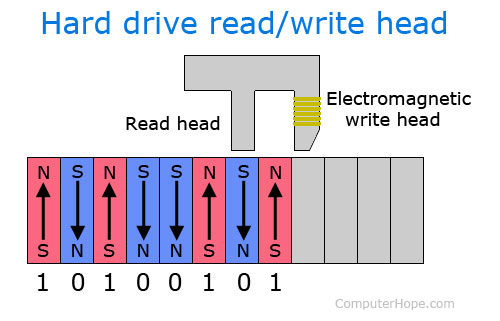
\includegraphics[scale = 0.40]{source/pictures/magnetic-media.jpg}
        \caption{Processo de gravação de dados em um disco rígido\cite{hdd-image}.}
        \label{fig:device}
    \end{figure}
%*----------- notes
    \note[item]{Notes can help you to remember important information. Turn on the notes option.}
\end{frame}

\begin{frame}[t]{Introdução}
    \transboxout[duration=0.5]
    \begin{columns}
        \column{.2\textwidth}
    \end{columns}

    \begin{block}{O que é \textit{Building Blocks}?}
        Unidades básicas de armazenamento do sistema de memória. É possível comparar a funcionalidade dos bits magnéticos com os bits mecânicos.
    \end{block}
    \only<2->{
    \begin{alertblock}{Mas, o que são esses bits mecânicos?}
    \end{alertblock}
    }
\end{frame}
